\documentclass[12pt,letter]{article}
\usepackage{../downey_format}


\begin{document}
	


	% set the section number, along with figure and equation numbers
	\setcounter{section}{5}	
	\setcounter{figure}{0}   
	\renewcommand\thefigure{\thesection.\arabic{figure}}
	\setcounter{equation}{0}   
	\renewcommand\theequation{\thesection.\arabic{equation}}


	\section{Support Vector Machines}








The core idea of Support Vector Machines becomes clear when viewed geometrically. Figure~\ref{fig:SVM_large_margin_classification} shows a slice of the iris dataset containing two linearly separable species. In the left panel two conventional linear classifiers are drawn; although both label every training point correctly, their separating lines sit very close to several observations, so even a small perturbation could lead to misclassifications on new data. The right panel plots the boundary produced by an SVM. The solid line still splits the classes cleanly, but it is positioned to maximise the distance to the nearest points, leaving the widest possible ``street'' (bounded by the dashed parallels). The samples that lie on these margins are the \emph{support vectors}. This strategy, called large margin classification, usually delivers models that generalise better than those that merely separate the training set.



\begin{figure}[H]
	\centering
	\includegraphics[width=6.5in]{../figures/SVM_large_margin_classification}
	\caption{Large margin classification.}
	\label{fig:SVM_large_margin_classification}
\end{figure}

Observe that the addition of further training instances outside the ``street'' does not influence the decision boundary; it is entirely shaped by the instances situated on the boundary's edge. These pivotal instances are termed support vectors and are highlighted with circles in Figure~\ref{fig:SVM_large_margin_classification}.




\begin{mdframed}[middlelinewidth=0.5mm]
\begin{center}
\bl{NOTE}
\end{center}
The sensitivity of SVMs to feature scales is evident in Figure~\ref{fig:SVM_feature_scaling}. In the left plot, the vertical dimension greatly outweighs the horizontal dimension, resulting in a nearly horizontal ``street.'' However, after applying feature scaling such as using Scikit-Learn's \texttt{StandardScaler} the decision boundary becomes more appropriate, as illustrated in the right plot.

\begin{figure}[H]
	\centering
	\includegraphics[width=6.0in]{../figures/SVM_feature_scaling}
	\caption{Sensitivity of support vectors to feature scaling. }
	\label{fig:SVM_feature_scaling}
\end{figure}

\end{mdframed}




\subsection{Linear SVM Classification}


Hard margin classification demands that all instances be correctly classified without any margin violations. This strict approach faces two significant challenges:
\begin{itemize}
    \item It is only feasible when the data is linearly separable.
    \item It is highly sensitive to outliers.
\end{itemize}
Figure~\ref{fig:SVM_hard_margin} illustrates these challenges using the iris dataset with an added outlier. On the left, achieving a hard margin is impossible due to the outlier. On the right, although a decision boundary is found, it deviates substantially from the optimal boundary shown in Figure~\ref{fig:SVM_large_margin_classification} and is less likely to perform well on new data.


\begin{figure}[H]
	\centering
	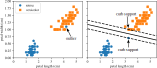
\includegraphics[width=6.5in]{../figures/SVM_hard_margin.png}
	\caption{Support vector machines showing (left) an un-separable case, and (right) a separable case with two data points supporting the curbs of the support vector machine. }
	\label{fig:SVM_hard_margin}
\end{figure}


To mitigate the limitations of hard margin classification, a more adaptable model, known as soft margin classification, is often employed. The goal here is to achieve an optimal balance between maximizing the margin width and minimizing margin violations, where instances might fall into the margin or on the incorrect side.

Scikit-Learn's SVM implementations facilitate this balance through the hyperparameter $C$. A smaller value of $C$ results in a wider margin but allows more margin violations, which is beneficial for model flexibility. Conversely, a larger $C$ value tightens the margin, reducing margin violations but at the risk of a less flexible model. Figure~\ref{fig:SVM_hyperparameter_C} demonstrates this trade-off: the left plot with a low $C$ value

\begin{figure}[H]
	\centering
	\includegraphics[width=6.5in]{../figures/SVM_hyperparameter_C.png}
	\caption{SVM margin sizes for different $C$ values.}
	\label{fig:SVM_hyperparameter_C}
\end{figure}


\begin{mdframed}[middlelinewidth=0.5mm]
\begin{center}
\bl{NOTE}
\end{center}
Overfitting in an SVM model can often be addressed by reducing the C value, which increases regularization.
\end{mdframed}


In earlier chapters we placed every model parameter in a single vector $\boldsymbol{\theta}$: the first entry $\theta_0$ acted as the bias, while $\theta_1,\dots,\theta_n$ were the feature weights, and each input was augmented with a constant bias feature $x_0 = 1$. In this chapter we adopt the notation most common for SVMs. The bias is written as $b$, the weight vector as $\mathbf{w}$, and no extra bias feature is appended to the input vectors.

\pagebreak

\subsubsection{Decision Function and Predictions}
A linear SVM classifier determines the class of a new instance $x$ by calculating the decision function
\begin{equation}
\textbf{w}^\text{T} \textbf{x} + b = w_1 x_1 + \cdots + w_n x_n + b.
\end{equation}
If the outcome is positive, the predicted class $\hat{y}$ is the positive class (1); otherwise, it is the negative class (0). This is written as 

\begin{equation}
  \hat{y} = 
  \begin{cases}
  0 & \text{if } \textbf{w}^\text{T} \textbf{x} + b < 0, \\
  1 & \text{if } \textbf{w}^\text{T} \textbf{x} + b \ge 0.
  \end{cases}
\label{eq:Linear_SVM_classifier_prediction}
\end{equation}

Figure~\ref{fig:SVM_decision_function} plots the decision function for a model with two features, so the surface is a plane in $\mathbb{R}^{2}$. The thick solid line marks the decision boundary where the function equals zero. The dashed lines show the loci where the function equals $1$ and $-1$; they run parallel to the boundary and sit at equal distance from it, outlining the margin. Training a linear SVM adjusts $\mathbf{w}$ and $b$ to make this margin as wide as possible while either prohibiting margin violations (hard margin) or keeping them small through a penalty term (soft margin).


\begin{figure}[H]
	\centering
	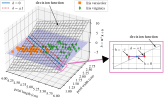
\includegraphics[]{../figures/SVM_decision_function}
	\caption{Decision function for the Iris Dataset showing how the decision function $h$ cuts through the feature space.}
	\label{fig:SVM_decision_function}
\end{figure}

\pagebreak

\subsubsection{Training Objective}

The slope of the decision function corresponds to the norm of the weight vector, $\|\textbf{w}\|$. Halving this slope causes the decision boundary margins, where the decision function equals $\pm 1$, to double in distance from the decision boundary. Effectively, reducing the norm of $\textbf{w}$ by half doubles the margin. This geometric interpretation is perhaps simpler to visualize in two dimensions, as shown in Figure~\ref{fig:SVM_weight_vectors}. Thus, minimizing $\|\textbf{w}\|$ maximizes the margin.

\begin{figure}[H]
	\centering
	\includegraphics[width=6.5in]{../figures/SVM_weight_vectors}
	\caption{The margin is dependent on the value of the weight vector where a smaller weight vector results in a larger margin and vise versa.}
	\label{fig:SVM_weight_vectors}
\end{figure}

To achieve a large margin while enforcing that no data points fall within the margin (hard margin), we ensure the decision function exceeds +1 for all positive training instances and is less than -1 for all negative instances. Let $t^{(i)}$ equal -1 for negative instances ($y^{(i)} = 0$) and +1 for positive ones ($y^{(i)} = 1$). The constraints then require
\begin{equation}
t^{(i)}(\textbf{w}^\text{T} \textbf{x}^{(i)} + b) \geq 1
\end{equation}
for all training instances. This forms the basis of the hard margin linear SVM classifier optimization problem:

\begin{equation}
\begin{split}
    & \underset{\textbf{w}, b}{\text{minimize}} \;\;\;\; \frac{1}{2}\textbf{w}^\text{T}\textbf{w} \\
    & \text{subject to} \;\;\;\; t^{(i)}(\textbf{w}^\text{T}\textbf{x}^{(i)} + b) \ge 1 \; \text{for} \; i = 1, 2, \ldots, m
\end{split}
\end{equation}


\begin{mdframed}[middlelinewidth=0.5mm]
\begin{center}
\bl{NOTE}
\end{center}
The objective function minimized is $\frac{1}{2}\textbf{w}^\text{T}\textbf{w}$, equivalent to $\frac{1}{2}\|\textbf{w}\|^2$. This formulation is chosen over minimizing $\|\textbf{w}\|$ directly because $\frac{1}{2}\|\textbf{w}\|^2$ offers a straightforward derivative, simply $\textbf{w}$, facilitating gradient calculations. In contrast, $\|\textbf{w}\|$ lacks differentiability at $\textbf{w} = 0$, posing challenges for optimization algorithms, which typically require smooth, differentiable functions to ensure effective optimization.
\end{mdframed}

To formulate the soft margin objective, it is necessary to introduce a slack variable $\zeta^{(i)} \geq 0$ for each instance. This variable, $\zeta^{(i)}$, quantifies the permissible margin violation for the i\textsuperscript{th} instance. Consequently, we face dual objectives: minimizing the slack variables to reduce margin violations and minimizing $\frac{1}{2}\textbf{w}^\text{T}\textbf{w}$ to maximize the margin. The hyperparameter $C$ plays a crucial role here, enabling a balance between these competing objectives. The introduction of $C$ transforms our task into a constrained optimization problem.

\begin{equation}
\begin{split}
    & \underset{\textbf{w}, b, \zeta}{\text{minimize}} \;\;\;\; \frac{1}{2}\textbf{w}^\text{T}\textbf{w} + C \sum_{i=1}^{m} \zeta^{(i)} \\  
    & \text{subject to} \;\;\;\; t^{(i)}(\textbf{w}^\text{T}\textbf{x}^{(i)}+b ) \ge 1 - \zeta^{(i)} \text{ and } \zeta^{(i)} \ge 0 \text{ for } i=1, \; 2, \; \cdots,  \; m 
\end{split}
\end{equation}

\subsubsection{Quadratic Programming}
Both hard margin and soft margin problems are examples of convex quadratic optimization problems with linear constraints, commonly referred to as Quadratic Programming (QP) problems. QP involves solving optimization problems where the objective is a quadratic function and the constraints are linear. This form of programming, established in the 1940s, predates and is distinct from ``computer programming,'' and is sometimes more descriptively termed ``quadratic optimization'' to avoid confusion.

A variety of techniques available through off-the-shelf solvers can address these QP problems, though they extend beyond the scope of this text. The general formulation of a QP problem is as follows:
\begin{equation}
\begin{split}
    & \underset{\textbf{p}}{\text{minimize}} \;\;\;\; \frac{1}{2}\textbf{\textbf{p}}^\text{T}\textbf{H}\textbf{p} + \textbf{f}^\text{T}\textbf{p}\\
    & \text{subject to} \;\;\;\; \textbf{A} \textbf{p} \le \textbf{b}
\end{split}
\label{eq:QP_problem}
\end{equation}
Here, $\textbf{p}$ is an $n_p$-dimensional vector (where $n_p$ is the number of parameters), $\textbf{H}$ is an $n_p \times n_p$ matrix, $\textbf{f}$ is an $n_p$-dimensional vector, $\textbf{A}$ is an $n_c \times n_p$ matrix (with $n_c$ being the number of constraints), and $\textbf{b}$ is an $n_c$-dimensional vector. 

Equation~\ref{eq:QP_problem} defines a standard quadratic program with constraints of the form $\textbf{A} \textbf{p} \le \textbf{b}$. For training a hard margin linear SVM, this setup can be used by choosing parameters that encode the SVM objective and constraints. The solution vector $\textbf{p}$ contains both the bias term and the feature weights. Using this knowledge, a standard QP solver can be applied directly to find the optimal SVM classifier.



\begin{example}
\textbf{Support Vector Machine Classification}

This example applies a linear Support Vector Machine (SVM) classifier to distinguish Iris-Virginica flowers based on petal length and width. The decision boundary is derived after scaling the data, and margins are visualized. Misclassified instances within the margin are identified and marked. The model's performance is assessed using a confusion matrix and F1 score.
\end{example}

\pagebreak
\subsection{Nonlinear SVM Classification}

\begin{figure}[H]
	\centering
	\includegraphics[width=6.5in]{../figures/nonlinear_SVM_example_illustration}
	\caption{Nonlinear SVM example illustration \protect\footnotemark[1]}
	\label{fig:nonlinear_SVM_example_illustration}
\end{figure}
\footnotetext[1]{Machine Learner, CC BY-SA 4.0 $<$https://creativecommons.org/licenses/by-sa/4.0$>$, via Wikimedia Commons}

While linear SVM classifiers are quite effective and perform exceptionally well in various scenarios, many datasets are far from being linearly separable. One strategy to address non-linear datasets is to introduce additional features, such as polynomial feature. Adding features can sometimes transform the dataset into one that is linearly separable. A representation of this technique is shown in \ref{fig:nonlinear_SVM_example_illustration}.

A simple example of converting non-linearly separable variables is shown in figure~\ref{fig:SVM_higher_dimensions} where the left plot displays a simple dataset with a single feature $x_1$. Clearly, this dataset is not linearly separable. However, by adding another feature $x_2 = (x_1)^2$, the dataset becomes perfectly linearly separable in two dimensions.

\begin{figure}[H]
	\centering
	\includegraphics[width=6.5in]{../figures/SVM_higher_dimensions.png}
	\caption{Illustration of SVM in higher dimensions}
	\label{fig:SVM_higher_dimensions}
\end{figure}

You can implement this idea in Scikit-Learn by creating a pipeline that applies a Polynomial Features transformer (introduced in the Regression Chapter), followed by a \texttt{StandardScaler} and a \texttt{LinearSVC}. The approach works nicely on the moons dataset, a toy binary-classification problem in which the samples trace two interleaving half-circles, as illustrated in Figure~\ref{fig:SVM_polynomial_features}. You can generate this dataset with the function \texttt{make\_moons()}.

\begin{figure}[H]
	\centering
	\includegraphics[width=6.5in]{../figures/SVM_polynomial_features.png}
	\caption{Demonstration of a SVM classifier with polynomial features.}
	\label{fig:SVM_polynomial_features}
\end{figure}

\begin{example}
\textbf{Nonlinear Classification}

\noindent This example demonstrates nonlinear classification leveraging \texttt{LinearSVC} in a pipeline with \texttt{preprocessing.PolynomialFeatures} using the \texttt{make\_moons} dataset. A polynomial feature transformation is combined with a linear SVM to classify the data, and the resulting decision boundaries are visualized.
\end{example}


\subsubsection{Kernel trick}

% \todo{Add text on Kernal math if needed}
While adding polynomial features is straightforward and enhances the performance of various Machine Learning algorithms (not limited to SVMs), it presents limitations. Specifically, lower-degree polynomials may not adequately handle complex datasets, and higher-degree polynomials significantly increase the feature count, slowing down the model.

SVMs offer a unique solution through a remarkable mathematical technique known as the kernel trick, which allows for the benefits of high-degree polynomial features without actually expanding the feature space, thereby avoiding a rapid increase in computation. This kernel trick is incorporated within the SVC class. 

In the dual form of an SVM the explicit dot product of two input vectors  
\begin{equation}
\mathbf x^{\mathrm T}\mathbf z
\end{equation} 
is replaced by a kernel function  
\begin{equation}
k(\mathbf x,\mathbf z),
\end{equation}
where $\mathbf x$ and $\mathbf z$ are $n$-dimensional feature vectors representing any two data points in the training set.  
This substitution lets the algorithm construct a linear separator in a (possibly infinite-dimensional) feature space while all calculations still occur in the original input coordinates.


%In the dual form of an SVM the inner product $\mathbf w^\text{T}\mathbf x$ is replaced by a kernel
%\begin{equation}
%k(\mathbf x,\mathbf x),
%\end{equation}
%allowing the algorithm to fit a \textit{linear} separator in a (possibly infinite-dimensional) feature space while the optimisation still takes place in the original coordinates. 

Figure~\ref{fig:SVM_polynomial_kernel} shows configured SVM classifiers using a 3\textsuperscript{rd} and 3\textsuperscript{th} degree polynomial kernel; on the left and right respectively. Adjusting the polynomial degree can help manage model fit: reducing the degree may prevent overfitting, whereas increasing it may be necessary for underfitting scenarios. The `coef0` hyperparameter is crucial as it determines the influence of high versus low-degree polynomials in the model.

\begin{mdframed}[middlelinewidth=0.5mm]
\begin{center}
\bl{NOTE}
\end{center}
A typical method for determining optimal hyperparameter settings involves utilizing grid search techniques. Starting with a broad, coarse grid search to quickly narrow down potential candidates, followed by a more detailed, finer grid search centered on these promising values often yields faster results. Additionally, understanding the function and influence of each hyperparameter aids in efficiently targeting the most relevant areas of the hyperparameter space.
\end{mdframed}


\begin{figure}[H]
	\centering
	\includegraphics[width=6.5in]{../figures/SVM_polynomial_kernel.png}
	\caption{SVM polynomial kernel}
	\label{fig:SVM_polynomial_kernel}
\end{figure}


\subsubsection{Standard Kernels}


Three kernels cover the vast majority of practical cases. 
\begin{itemize}
\item The polynomial kernel captures interactions between input features up to a chosen degree~$d$:
\begin{equation}
k_{\text{poly}}\bigl(\textbf{x},\textbf{z}\bigr)
  = \bigl(\textbf{x}^{\text{T}}\textbf{z} + c\bigr)^{d}
\end{equation}
where $c\!\ge\!0$ is a constant offset.  It is effective when domain knowledge suggests that a low-order combination of variables explains the target.  Keep $d$ modest (typically $d\le5$) and standardise inputs to avoid exploding feature dimensions and overfitting.
\item The radial basis function (RBF) kernel builds smooth, highly flexible decision boundaries:
\begin{equation}
k_{\text{rbf}}\bigl(\textbf{x},\textbf{z}\bigr)
  = \exp\!\bigl(-\gamma \lVert \textbf{x}-\textbf{z}\rVert^{2}\bigr)
\end{equation}
with width parameter $\gamma>0$.  A large $\gamma$ makes the surface too flat (underfitting), while a small $\gamma$ lets every point carve its own pocket (overfitting).  Tune $C$ and $\gamma$ jointly, typically on a logarithmic grid, after x-score standardising the features.
\item The sigmoid kernel adds an S-shaped non-linearity to the inner product:
\begin{equation}
k_{\text{sig}}\bigl(\textbf{x},\textbf{z}\bigr)
  = \tanh\!\bigl(\kappa\,\textbf{x}^{\text{T}}\textbf{z} + \theta\bigr)
\end{equation}
where $\kappa$ controls the slope and $\theta$ the offset.  Although useful for some sparse or text data, this kernel is not always positive-semidefinite, so ensure your software handles the resulting optimisation safely.
\end{itemize}

\begin{example}
\textbf{Polynomial Kernel Trick}

\noindent This example uses the kernel trick to enable an SVM to classify non-linearly separable data using \texttt{SVC} (not \texttt{LinearSVC}). A third-degree polynomial kernel is applied to the moons dataset using Scikit-Learn's \texttt{Pipeline} and \texttt{SVC} tools, producing a curved decision boundary that cleanly separates the classes.
\end{example}


\begin{mdframed}[middlelinewidth=0.5mm]
\begin{center}
\bl{NOTE}
\end{center}
Begin with the RBF kernel as a strong default, explore polynomial kernels when you expect specific interaction orders, and treat the sigmoid option as experimental unless you have evidence it helps.
\end{mdframed}

\subsection{Computational Complexity}

Scikit-Learn provides two main SVM classifiers that trade accuracy for speed in different ways.  
\texttt{LinearSVC} is optimized for large, high-dimensional data when a linear decision boundary is adequate; \texttt{SVC} sacrifices runtime for the expressive power of kernels and thus handles complex, nonlinear patterns. Table \ref{table:SVM_classifiers} highlights how these priorities translate into computational costs and practical constraints and compares them to \texttt{SGDClassifier} for reference.

% Please add the following required packages to your document preamble:
% \usepackage{booktabs}
\begin{table}[H]
\caption{Key characteristics of three Scikit-Learn SVM classifier implementations.}
\label{table:SVM_classifiers}
\begin{tabular}{@{}lllll@{}}
Trule
class & time complexity & out-of-core support & scaling required & kernel trick \\ \midrule
\texttt{LinearSVC} & $O(m \times n)$ & no & yes & no \\
\texttt{SVC} & $O(m^2 \times n)$ to $O(m^3 \times n)$ & no & yes & yes \\
\texttt{SGDClassifier} & $O(m \times n)$ & yes & yes & no \\ \bottomrule
\end{tabular}
\end{table}


\texttt{LinearSVC} builds on the \texttt{liblinear} solver and is limited to \emph{linear} decision boundaries.  
Because it does not apply the kernel trick, its training cost grows almost linearly with both the number of samples~\(m\) and features~\(n\), i.e.\ \(O(m\,n)\). Convergence is controlled by the tolerance parameter \texttt{tol} (denoted \(\epsilon\) in the literature); the default value is usually sufficient, but smaller tolerances can be specified when higher accuracy is critical.

\texttt{SVC}, in contrast, relies on \texttt{libsvm} and \emph{does} support kernel functions. Its computational burden is markedly heavier, between \(O(m^{2} n)\) and \(O(m^{3} n)\) in practice, so training becomes prohibitive once the dataset reaches the hundreds-of-thousands range. Nevertheless, \texttt{SVC} excels on smaller or medium-sized problems that demand nonlinear decision surfaces. Runtime also scales with the average count of non-zero features per instance, meaning sparse high-dimensional inputs remain tractable. 





\vspace{-1ex}
\subsection{SVM Regression}
\label{sec:svr}
\vspace{-1ex}

Support Vector Regression (SVR) adapts the SVM idea to regression by surrounding the prediction curve with a tube of width $\epsilon$; points outside this tube incur a penalty and the optimizer keeps the tube as flat as possible while allowing a limited number of violations governed by the regularization constant $C$.  Conceptually this reverses the classification goal: instead of widening a margin to separate two classes, SVR encourages the data to lie inside the margin, making $\epsilon$ the principal knob that controls how loose the fit may be for both linear and kernel-based models.





\subsubsection{Linear SVR}
\vspace{-1ex}
The presence of additional training instances within the margin does not influence the predictions of the model, rendering it $\epsilon$-insensitive. For linear SVM Regression tasks, the LinearSVR class from Scikit-Learn can be utilized. For instance, 
Figure~\ref{fig:SVM_Regression} demonstrates two linear SVM Regression models trained on random linear data; one features a wide margin ($\epsilon = 1.5$), and the other a narrower margin ($\epsilon = 0.5$).

\begin{figure}[H]
	\centering
	\vspace{-1ex}
	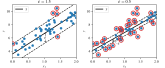
\includegraphics[width=6.5in]{../figures/SVM_Regression.png}
\vspace{-2ex}
	\caption{SVM Regression models with different $\epsilon$ values.}
	\label{fig:SVM_Regression}
\end{figure}

For data that follow an approximately linear trend, the \texttt{LinearSVR} class in Scikit-Learn solves the primal problem directly. It scales in $O(mn)$ time with $m$ samples and $n$ features, making it a practical choice for large data sets where a simple linear fit is adequate.

\subsubsection{Kernel SVR}
\label{sec:svr-kernel}
When the relationship is non-linear, the \texttt{SVR} class employs the kernel trick:
\begin{equation}
f(x)=\sum_{i=1}^{m}(\alpha_i-\alpha_i^{\!*})\,k(x_i,x)+b,
\end{equation}
where $k(\cdot,\cdot)$ is typically RBF or polynomial.  Figure~\ref{fig:SVM_regression_2nd_degree} shows a 2\textsuperscript{nd}-degree polynomial kernel
capturing quadratic structure under various regularisation levels.

The Scikit-lern SVR class, supporting the kernel trick and acting as the regression counterpart to the SVC class, performs well with small to medium-sized datasets but slows considerably as dataset size increases. In contrast, the LinearSVR class, akin to the LinearSVC class, scales linearly with the size of the training set.

\begin{figure}[H]
	\centering
	\includegraphics[width=6.5in]{../figures/SVM_regression_2nd_degree.png}
	\caption{SVM regression with a 2\textsuperscript{nd}-degree polynomial kernel, showcasing different regularization levels.}
	\label{fig:SVM_regression_2nd_degree}
\end{figure}


\begin{example}
\textbf{SVM Polynomial Regression}

This example fits a non-linear regression curve to noisy quadratic data using Support Vector Regression (SVR) with a polynomial kernel. It highlights how SVR models can handle non-linear relationships by introducing a margin of tolerance.
\end{example}

\pagebreak
\includepdf[pages=1, width= 0.95\textwidth, pagecommand = {\subsection{Examples} \subsubsection*{Example 6.1}\vspace{0.5em}}]{../code/example_6.1_Linear_Classification.pdf}
\includepdf[pages=2, width= 0.95\textwidth, pagecommand = {\vspace{0.5em}}]{../code/example_6.1_Linear_Classification.pdf}

\includepdf[pages=1, width= 0.95\textwidth, pagecommand = {\subsubsection*{Example 6.2}\vspace{0.5em}}]{../code/example_6.2_polynomial_features.pdf}


\includepdf[pages=1, width= 0.95\textwidth, pagecommand = {\subsubsection*{Example 6.3}\vspace{0.5em}}]{../code/example_6.3_SVM_Polynomial_kernel.pdf}


\includepdf[pages=1, width= 0.95\textwidth, pagecommand = {\subsubsection*{Example 6.4}\vspace{0.5em}}]{../code/example_6.4_SVM_regression.pdf}









































\end{document}

